% !TEX root = ../../prj4projektdokumentation.tex
% SKAL STÅ I TOPPEN AF ALLE FILER FOR AT MASTER-filen KOMPILERES 

\section{Allokeringsdiagram}
På figur \ref{fig:Allokering} ses allokeringsdiagram for spændningsregulatoren. Diagrammet er lavet for at danne overblik over softwaren, derfor er analog moduler undladt. Styringsenheden laver et output til trin transformeren og Måleenehederne får input fra belastninger. Det er heller ikke vist på diagrammet. Diagrammet viser hvilke platforme de logiske blokke skal laves på, og hvordan kommunikationen er mellem blokkene

\begin{enumerate}
	\item Styringsenheden allokeres på en PLC
	\item Brugergrænsefladen allokeres på en HMI skærm
	\item Måleenhederne allokeres på PSoCs
\end{enumerate}   

\begin{figure}[htbp] % (alternativt [H])
	\centering
	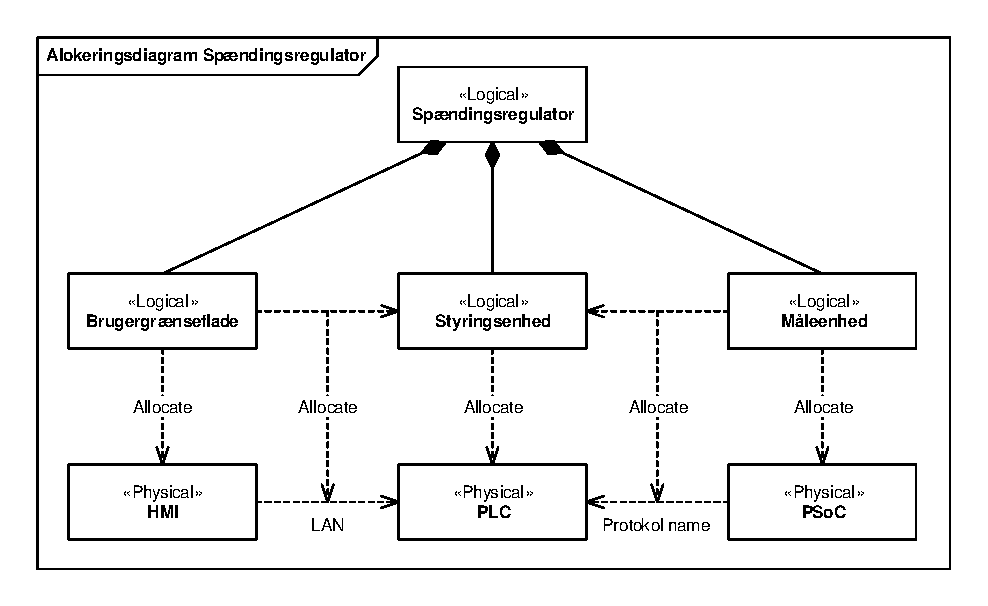
\includegraphics[width=0.9\textwidth]{Figure/Allokering}
	\caption{Allokeringsdiagram for spændingsregulator}
	\label{fig:Allokering}
\end{figure}